% Options for packages loaded elsewhere
\PassOptionsToPackage{unicode}{hyperref}
\PassOptionsToPackage{hyphens}{url}
\PassOptionsToPackage{dvipsnames,svgnames,x11names}{xcolor}
%
\documentclass[
  letterpaper,
  DIV=11,
  numbers=noendperiod]{scrartcl}

\usepackage{amsmath,amssymb}
\usepackage{iftex}
\ifPDFTeX
  \usepackage[T1]{fontenc}
  \usepackage[utf8]{inputenc}
  \usepackage{textcomp} % provide euro and other symbols
\else % if luatex or xetex
  \usepackage{unicode-math}
  \defaultfontfeatures{Scale=MatchLowercase}
  \defaultfontfeatures[\rmfamily]{Ligatures=TeX,Scale=1}
\fi
\usepackage{lmodern}
\ifPDFTeX\else  
    % xetex/luatex font selection
\fi
% Use upquote if available, for straight quotes in verbatim environments
\IfFileExists{upquote.sty}{\usepackage{upquote}}{}
\IfFileExists{microtype.sty}{% use microtype if available
  \usepackage[]{microtype}
  \UseMicrotypeSet[protrusion]{basicmath} % disable protrusion for tt fonts
}{}
\makeatletter
\@ifundefined{KOMAClassName}{% if non-KOMA class
  \IfFileExists{parskip.sty}{%
    \usepackage{parskip}
  }{% else
    \setlength{\parindent}{0pt}
    \setlength{\parskip}{6pt plus 2pt minus 1pt}}
}{% if KOMA class
  \KOMAoptions{parskip=half}}
\makeatother
\usepackage{xcolor}
\setlength{\emergencystretch}{3em} % prevent overfull lines
\setcounter{secnumdepth}{-\maxdimen} % remove section numbering
% Make \paragraph and \subparagraph free-standing
\ifx\paragraph\undefined\else
  \let\oldparagraph\paragraph
  \renewcommand{\paragraph}[1]{\oldparagraph{#1}\mbox{}}
\fi
\ifx\subparagraph\undefined\else
  \let\oldsubparagraph\subparagraph
  \renewcommand{\subparagraph}[1]{\oldsubparagraph{#1}\mbox{}}
\fi


\providecommand{\tightlist}{%
  \setlength{\itemsep}{0pt}\setlength{\parskip}{0pt}}\usepackage{longtable,booktabs,array}
\usepackage{calc} % for calculating minipage widths
% Correct order of tables after \paragraph or \subparagraph
\usepackage{etoolbox}
\makeatletter
\patchcmd\longtable{\par}{\if@noskipsec\mbox{}\fi\par}{}{}
\makeatother
% Allow footnotes in longtable head/foot
\IfFileExists{footnotehyper.sty}{\usepackage{footnotehyper}}{\usepackage{footnote}}
\makesavenoteenv{longtable}
\usepackage{graphicx}
\makeatletter
\def\maxwidth{\ifdim\Gin@nat@width>\linewidth\linewidth\else\Gin@nat@width\fi}
\def\maxheight{\ifdim\Gin@nat@height>\textheight\textheight\else\Gin@nat@height\fi}
\makeatother
% Scale images if necessary, so that they will not overflow the page
% margins by default, and it is still possible to overwrite the defaults
% using explicit options in \includegraphics[width, height, ...]{}
\setkeys{Gin}{width=\maxwidth,height=\maxheight,keepaspectratio}
% Set default figure placement to htbp
\makeatletter
\def\fps@figure{htbp}
\makeatother

\KOMAoption{captions}{tableheading}
\makeatletter
\@ifpackageloaded{caption}{}{\usepackage{caption}}
\AtBeginDocument{%
\ifdefined\contentsname
  \renewcommand*\contentsname{Table of contents}
\else
  \newcommand\contentsname{Table of contents}
\fi
\ifdefined\listfigurename
  \renewcommand*\listfigurename{List of Figures}
\else
  \newcommand\listfigurename{List of Figures}
\fi
\ifdefined\listtablename
  \renewcommand*\listtablename{List of Tables}
\else
  \newcommand\listtablename{List of Tables}
\fi
\ifdefined\figurename
  \renewcommand*\figurename{Figure}
\else
  \newcommand\figurename{Figure}
\fi
\ifdefined\tablename
  \renewcommand*\tablename{Table}
\else
  \newcommand\tablename{Table}
\fi
}
\@ifpackageloaded{float}{}{\usepackage{float}}
\floatstyle{ruled}
\@ifundefined{c@chapter}{\newfloat{codelisting}{h}{lop}}{\newfloat{codelisting}{h}{lop}[chapter]}
\floatname{codelisting}{Listing}
\newcommand*\listoflistings{\listof{codelisting}{List of Listings}}
\makeatother
\makeatletter
\makeatother
\makeatletter
\@ifpackageloaded{caption}{}{\usepackage{caption}}
\@ifpackageloaded{subcaption}{}{\usepackage{subcaption}}
\makeatother
\ifLuaTeX
  \usepackage{selnolig}  % disable illegal ligatures
\fi
\usepackage{bookmark}

\IfFileExists{xurl.sty}{\usepackage{xurl}}{} % add URL line breaks if available
\urlstyle{same} % disable monospaced font for URLs
\hypersetup{
  pdftitle={Homework 2},
  pdfauthor={Kelsey Hawkins},
  colorlinks=true,
  linkcolor={blue},
  filecolor={Maroon},
  citecolor={Blue},
  urlcolor={Blue},
  pdfcreator={LaTeX via pandoc}}

\title{Homework 2}
\author{Kelsey Hawkins}
\date{}

\begin{document}
\maketitle

\section{Introduction}\label{introduction}

ASL is a prominent language in the American deaf community. With this in
mind, I have a dataset of images containing the ASL dictionary,
excluding the letters that need motion. The dataset was already
flattened into greyscale values, ready for model input with a few
preprocessing changes. This model will help translate ASL images to text
for those who do not understand it, or want to learn it.

\section{Analysis}\label{analysis}

The first exploratory item I did was visualizing a few images from the
dataset. Not only did I want to ensure the data accuracy, but I wanted
to see what resolution I was working with. It was hard to do any summary
statistics or heatmaps, etc. due to the data being flattened images so
no EDA would have been useful in this case.

However, the images have a 28 x 28 x 1 size, a very low resolution image
of hands depicting each letter of the american alphabet. Since the
images have been flattened into columns of greyscale values, there will
be 784 columns, and all values except for the predictor variable were
scaled between 0-1. The predictor variable is a single number that
denotes a letter of the alphabet, excluding J and Z which require
motion.

\begin{verbatim}
(27455, 784) (27455, 24)
(7172, 784) (7172, 24)
\end{verbatim}

\begin{figure}

{\centering 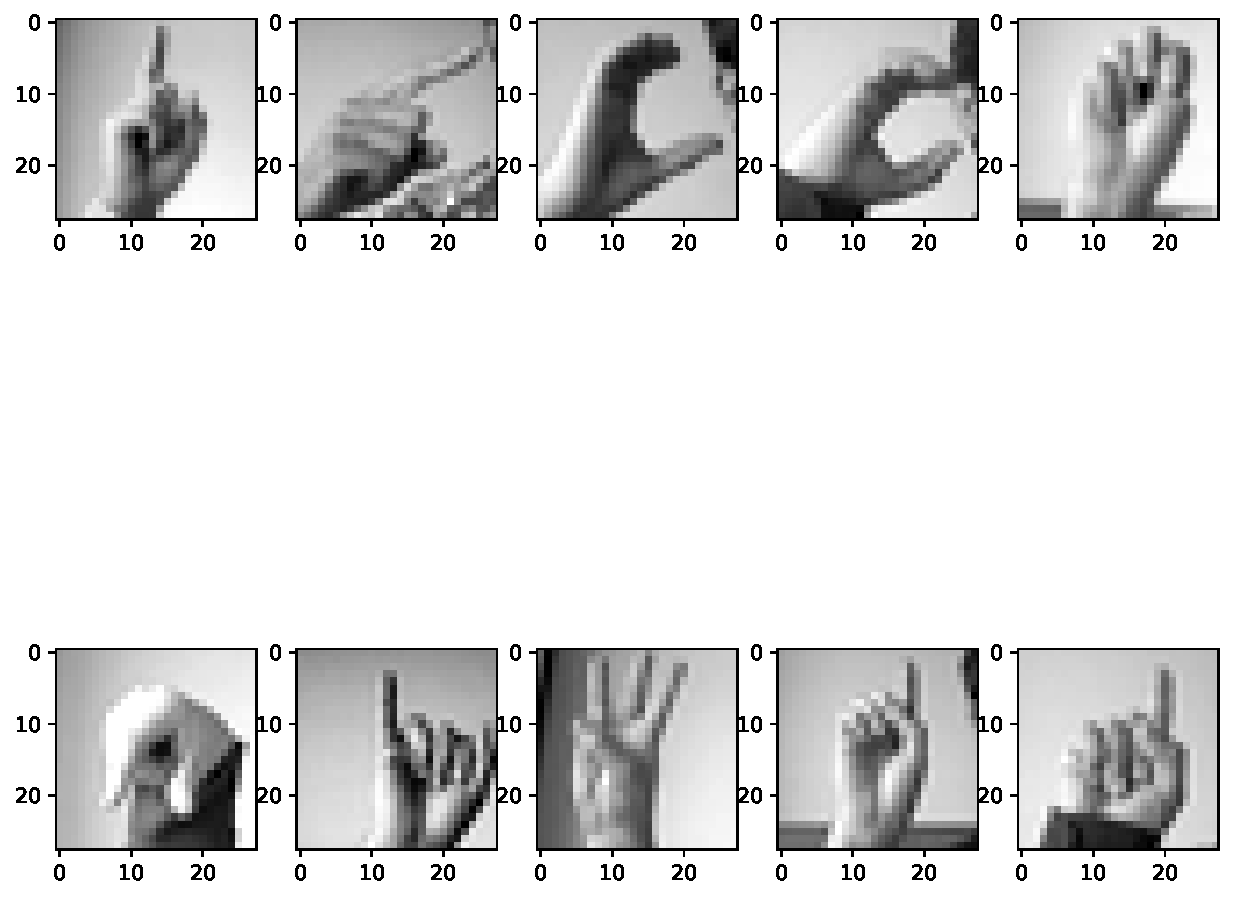
\includegraphics{HW2_Reflection_files/figure-pdf/random-images-from-dataset-output-2.pdf}

}

\caption{Random Images from Dataset}

\end{figure}%

\section{Methods}\label{methods}

The first model I created is a Deep Feed-Forward Neural Network. I
started with a simple model, built in class that had about 6 hidden
layers. I then expanded it by adding more dropout, dense, and batch
normalization layers. Each dense layer has an activation function of
reLU, and a kernel regularizer of L2 on two early dense layers. The last
dense layer outputs 24 nodes with a softmax activation function for
predicted probabilities for each letter. When I compiled my model, I
tested multiple optimizers including SGD, Adam, and RMSprop. The model
included early stopping to prevent overfitting.

The second model I created is a Random Forest Classifier. I created a
simple one to get a general sense of the model outputs and comparison to
the DNN. Then, I built a tuned RFC by utilizing the Randomized Search CV
module. The parameters I tuned were the number of estimators, max depth,
min samples split and leaf. The scorers were a combination of accuracy
and F1 for a combination between all three classification metrics.

\section{Results}\label{results}

With my two models, it is proven that deep learning is not needed. In
the deep neural network, no matter how many layers I added or removed,
or tuning I did, the metrics did not significantly improve. Both the
accuracy and F1 scores were extremely low and the model failed to fit to
the data well. Especially since I could not use convolutional layers,
the neural network failed to find features well. The training and
testing scores were not far from eachother, so no underfitting or
overfitting was present. However, the testing accuracy was 34\%, and the
F1 score was also 34\%.

\begin{figure}

{\centering 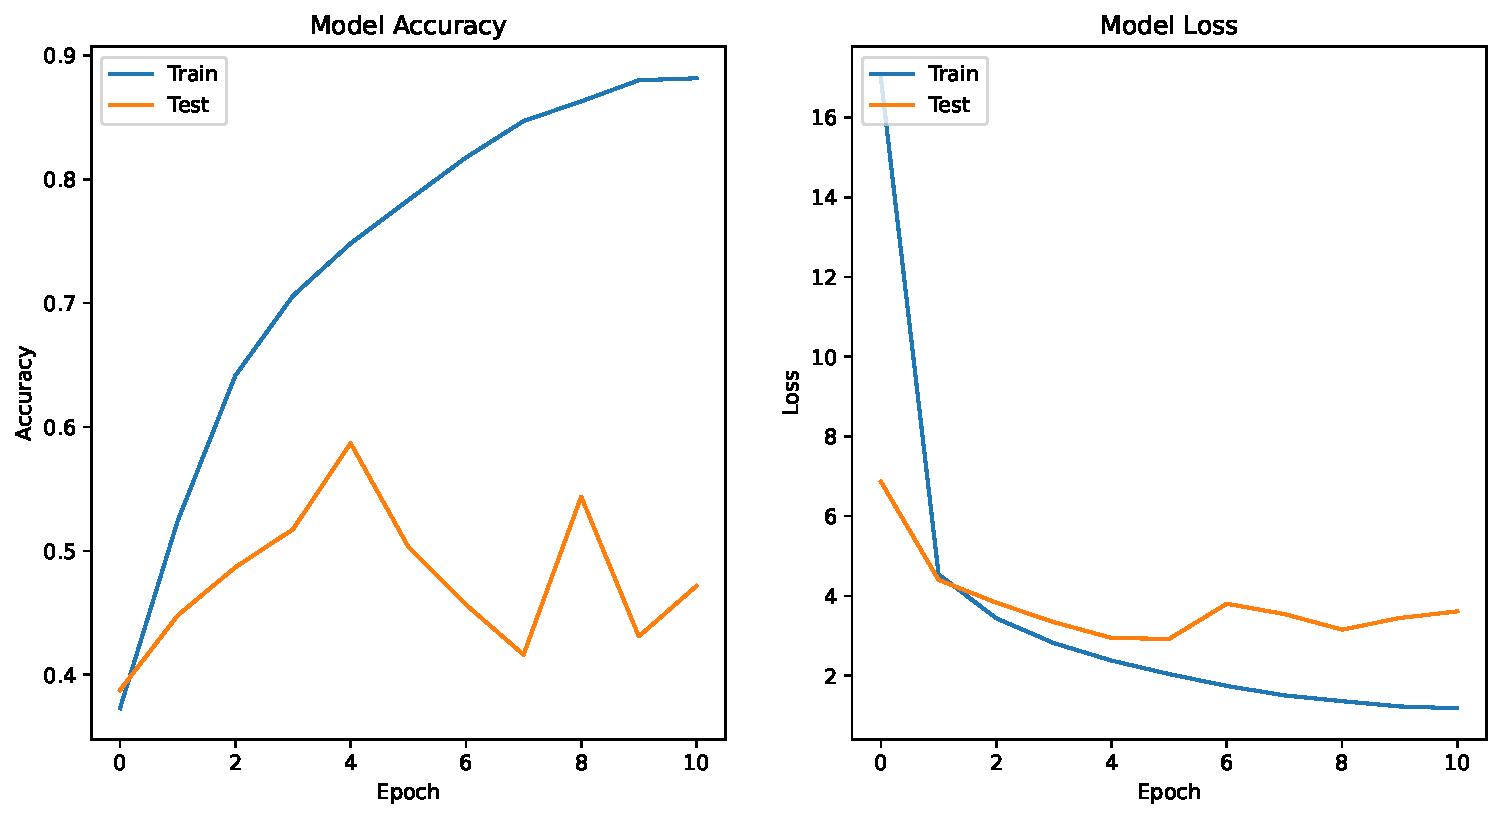
\includegraphics{HW2_Reflection_files/figure-pdf/model_output_dnn_graph-output-1.pdf}

}

\caption{Model validation and test over epochs}

\end{figure}%

\begin{verbatim}
  1/225 ━━━━━━━━━━━━━━━━━━━━ 7s 32ms/step 90/225 ━━━━━━━━━━━━━━━━━━━━ 0s 566us/step192/225 ━━━━━━━━━━━━━━━━━━━━ 0s 527us/step225/225 ━━━━━━━━━━━━━━━━━━━━ 0s 636us/step
\end{verbatim}

\begin{figure}

{\centering 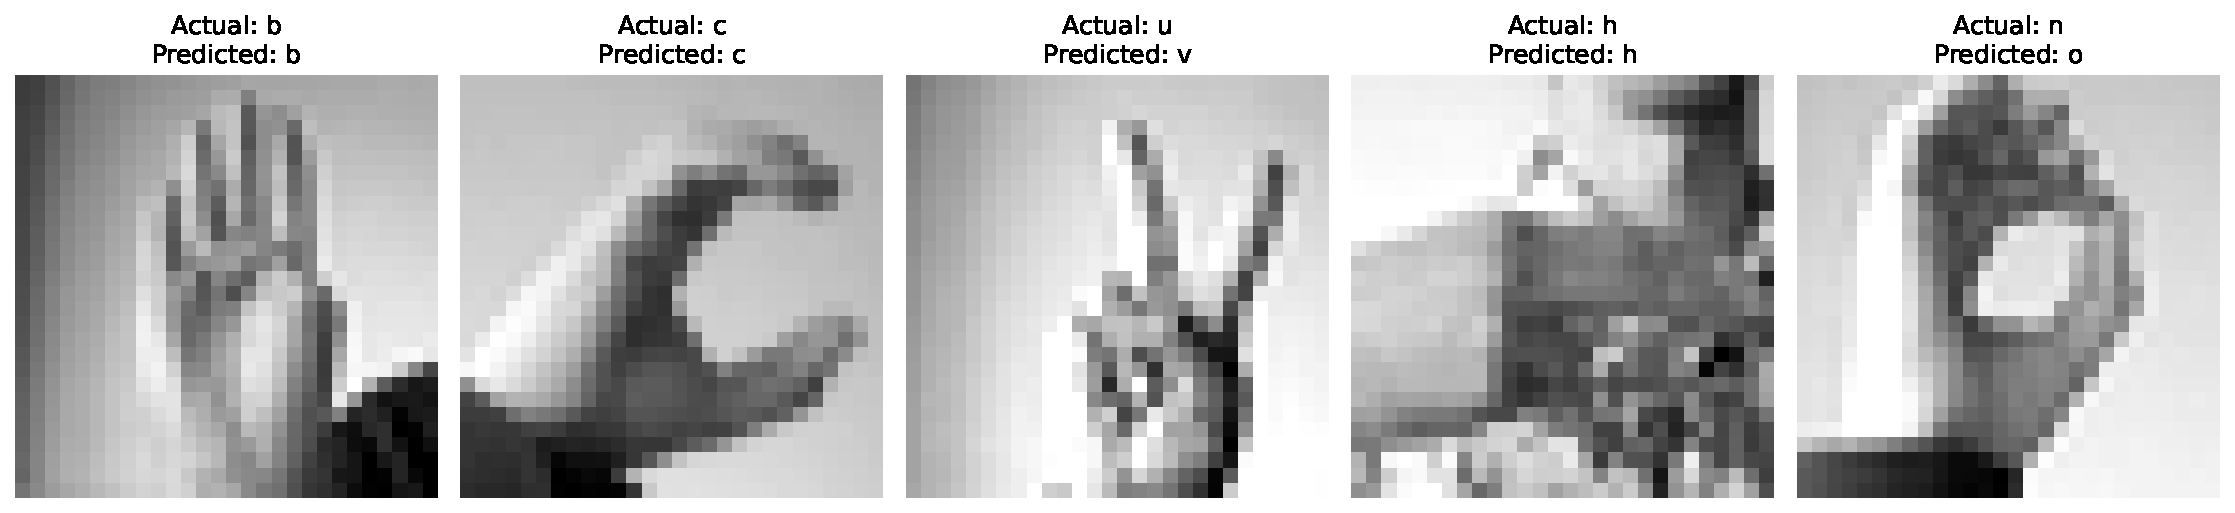
\includegraphics{HW2_Reflection_files/figure-pdf/model_output_dnn_images-output-2.pdf}

}

\caption{DNN Predictions over Test Images}

\end{figure}%

In the random forest classifier model, the metrics were quite different
than the DNN. This further proves deep learning is not necessary in this
context as the comparison of scores were multitudes different. The
random forest classifier outputted very high metrics once it was tuned.
The tuner found the best number of estimators to be 300, the min samples
split of 2, and min samples leaf to be 1 and max depth of 20. The
training and testing accuracy showed signs of overfitting as the
training accuracy was 100\% and the testing accuracy was 83\%. In the
images below, we can see the predictions were valid for all five images,
as opposed to the predictions made by the DNN.

\begin{verbatim}
Fitting 2 folds for each of 10 candidates, totalling 20 fits
Best parameters found:  {'n_estimators': 300, 'min_samples_split': 2, 'min_samples_leaf': 1, 'max_depth': 20}
\end{verbatim}

\begin{figure}

{\centering 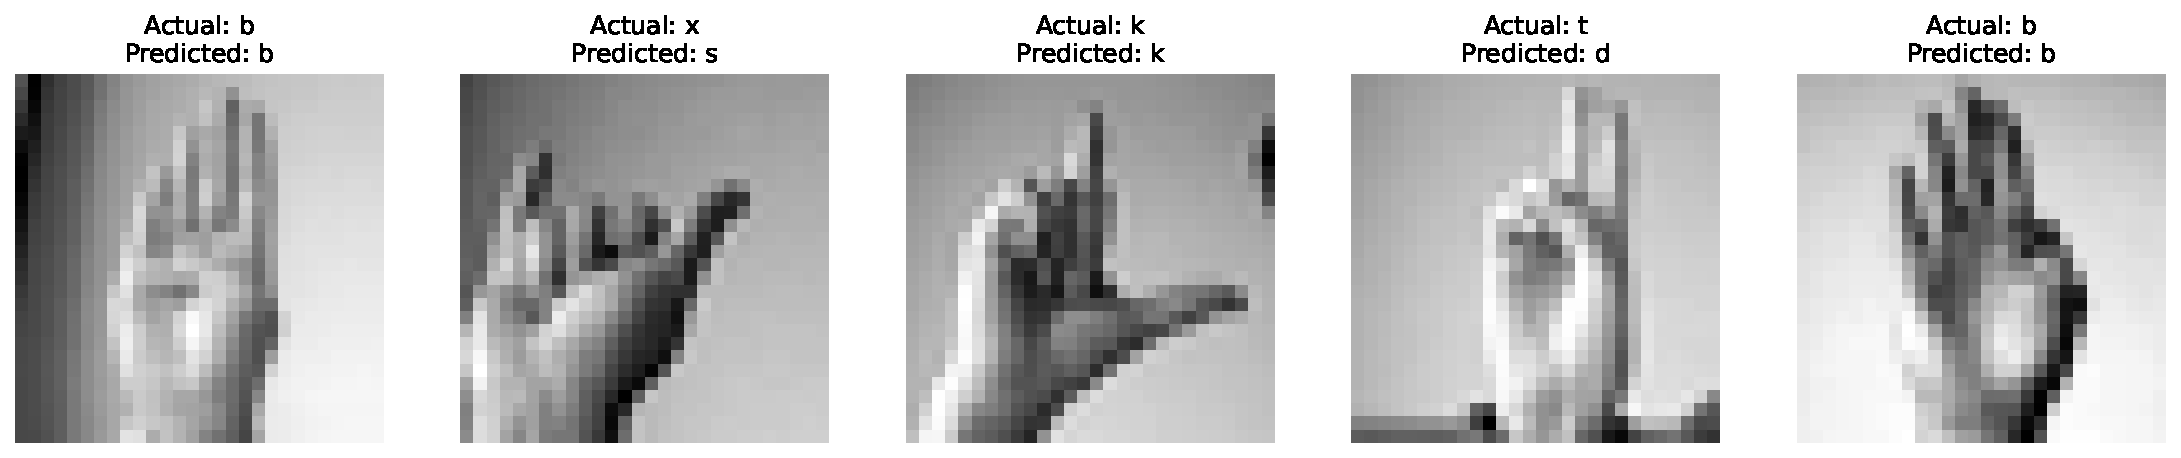
\includegraphics{HW2_Reflection_files/figure-pdf/model_output_rfc_images-output-2.pdf}

}

\caption{RFC Predictions over Test Images}

\end{figure}%

\section{Reflection}\label{reflection}

In this assignment, I did not come across many struggles or problems
with the code or analysis. However I did refer back to the math of the
models to justify my answers and think about why the models performed
the way they did. It was interesting to be able to quantify them with a
simple classification problem and think about how each model handles
class imbalances in the slightest way, by about 20\%. In the future, I
would approach it the same way as I did here, as it seemed to work well.



\end{document}
